%------------------------------%
%% ✎ Dylan (V1) %%%%%%%%% ✅ %%
%% ✎ Alain (V2) %%%%%%%%% ✅ %%
%% ✎ Dylan (V3) %%%%%%%%% ✅ %%
%------------------------------%

\afterpage{%
\afterpage{%

    % Arrière-plan partie III
    \AddToShipoutPictureBG*{%
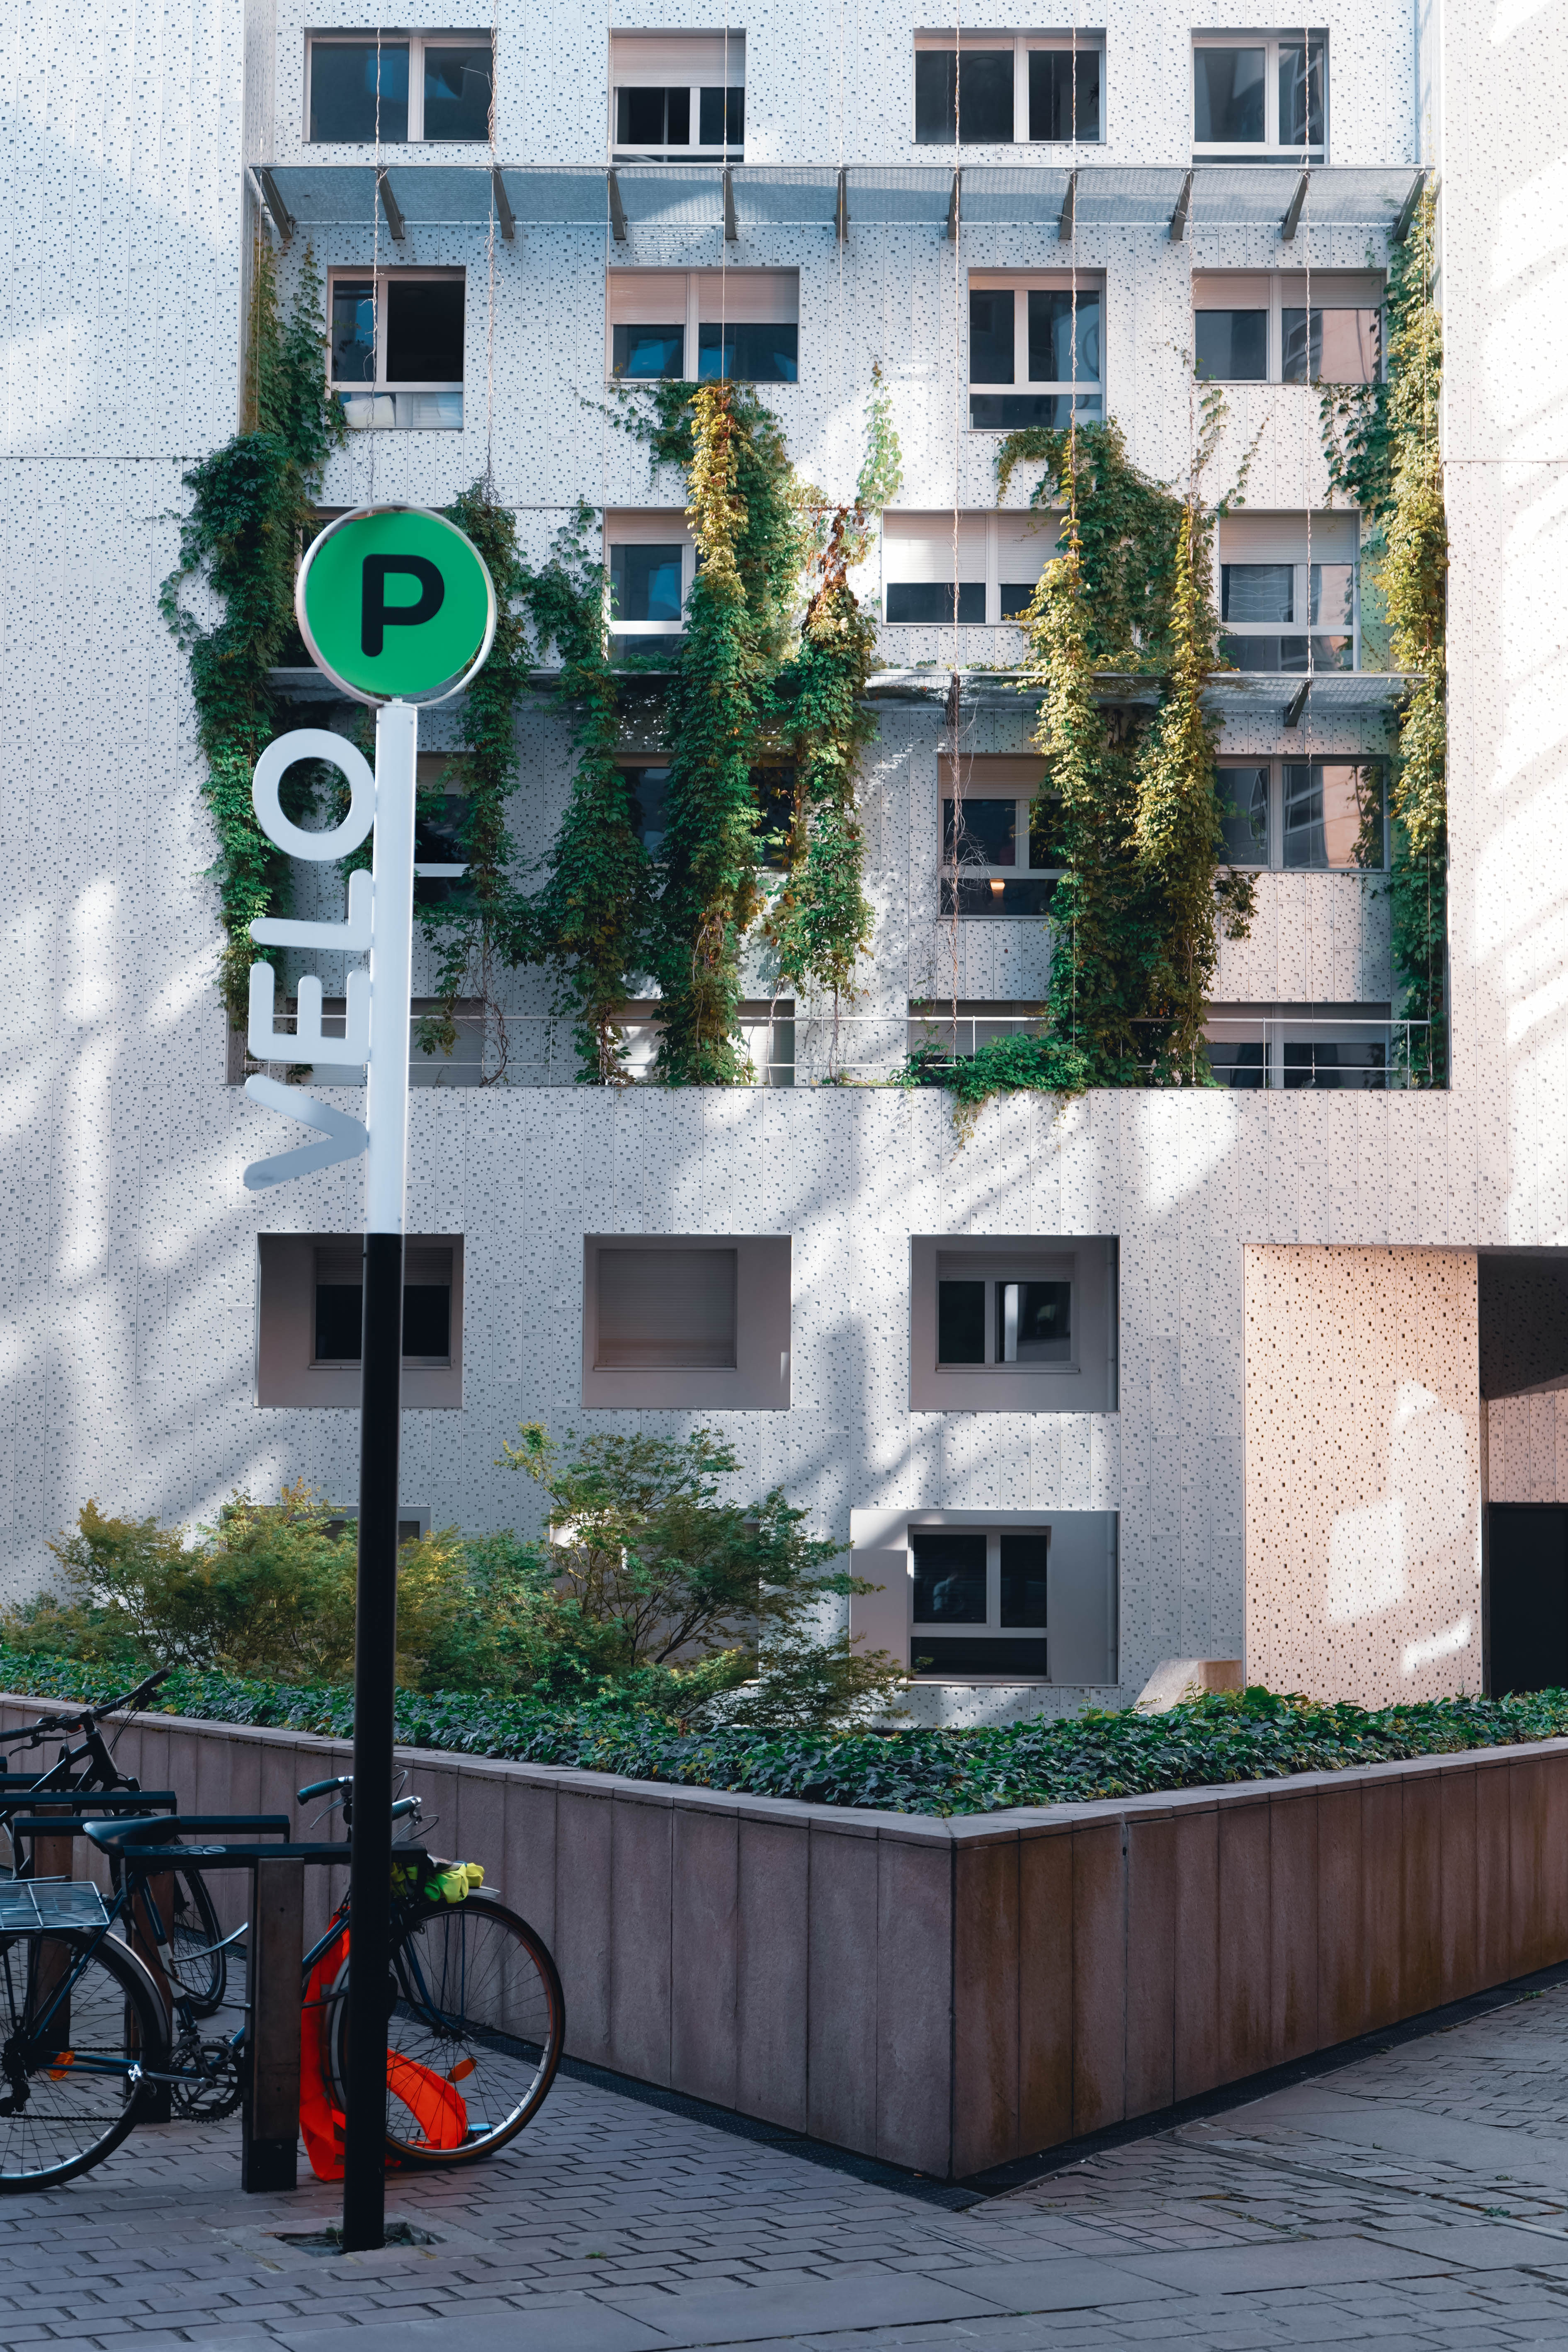
\includegraphics[width=\paperwidth,height=\paperheight]{src/Figures/Arriere_plan/Arriere_plan_Part_3.jpg}
    }

% Rectangle
\AddToShipoutPictureBG*{
  \begin{tikzpicture}[remember picture,overlay]
    \node[fill=white, opacity=0.75, text width=\paperwidth, minimum height=10cm, anchor=north] 
    at ([yshift=-7.7cm]current page.north) {};
  \end{tikzpicture}
}

% Source
\AddToShipoutPictureFG*{
  \AtPageLowerRight{
    \raisebox{1cm}{
      \hspace{16cm}
      
\begin{tikzpicture}
        \node[fill=white, rounded corners=5pt, inner sep=5pt, align=center] {
          \tiny{Photography: \textcolor{blue}{Dylan Moinse (2024)}}
        };
      \end{tikzpicture}
    }
  }
}
}}

\needspace{1\baselineskip} % Reserve space
\part{Practical Formalization of a Regional and Intermodal System, Rail-Oriented and Supported by Light Individual Mobility
    \label{part3:titre}
    }
    \markboth{Part~III: Functional Translation of \textsl{Micromobility-friendly Transit-Oriented Development}}{}
    \markright{Part~III: Functional Translation of \textsl{Micromobility-friendly Transit-Oriented Development}}{}

% Introduction of Part III
\cleardoublepage
\section*{Introduction of Part~III
    \label{part3:introduction}
    }
    \addcontentsline{toc}{chapter}{Introduction of Part~III}

    % Introduction
\lettrine[lines=3, findent=8pt, nindent=0pt]{\lettrinefont T}{he} conceptual and empirical analyses developed in the previous parts have highlighted the strategic role of light individual mobility in improving the intermodal accessibility of station districts and its potential to renew the \acrshort{TOD} model. They have shown that the integration of these mobility solutions, although promising, remains fragmented and insufficiently framed, both in terms of infrastructure and public policies. These findings underscore the need to formalize a theoretical and operational framework that structures the integration of individual mobility within an \acrshort{M-TOD}, in order to optimize its effectiveness and ensure a transition towards a more efficient, resilient, and inclusive intermodal urbanism. It is with this perspective that this third and final part aims to propose an expanded model of \acrshort{TOD}, which we refer to as \acrfull{M-TOD}, and which seeks to rethink the structuring of territories around public transport networks through a more adapted approach to the intermodal practices that have recently developed in the regions. These elements converge towards the same conclusion: the \acrshort{TOD}, in its current design, does not yet take into account the rise of new mobility solutions and must evolve to better integrate light individual mobility as a key element of its operation. This evolution is addressed by the formalization of \acrshort{M-TOD}.%%Translated%%

    % Chapter 6
\textsl{Formalizing a Micromobility-friendly Transit-Oriented Development that Systemically Integrates Light Individual Mobility in Station Districts} (\hyperref[objectif-6]{Objective~\(O_6\)}, page~\pageref{objectif-6}). \hyperref[chap6:titre]{The sixth chapter} (page~\pageref{chap6:titre}) focuses on formalizing the adaptation of the planning concept by translating it into urban strategies. It defines its guiding principles and identifies the conditions necessary for its successful implementation in urban planning and transport policies. This formalization relies on regional modeling, aiming to revisit the \acrfull{NPM} by integrating several dimensions: the forms of the network and the services of the rail system; the degree of urban development and the quality of the built environment; the connections and configuration of public spaces within station districts; and the temporal frequency of transit hubs. Such an approach, combining the strengths of geography and data science, leads us to identify and quantify the influence of various factors on the attractiveness of the public transport network. It also guides us in classifying stations and their surroundings into three intervention categories to be implemented, in line with the \acrshort{TOD} at the pedestrian scale and with the \acrshort{M-TOD} at the cycling scale. This modeling work is complemented by a case study on a rail corridor, allowing the operational implications of the reinterpreted model to be transposed. The analysis of these elements results in the proposal of a strategic roadmap, articulating actions and recommendations to sustainably incorporate light individual mobility into transport and urban planning.%%Translated%%
